% -------------------------------------------------
%
% Mobile Human-Computer Interaction
%
%   2019-2020 Coursework Template
%
\documentclass[a4,10pt,twocolumn]{article}

\usepackage[margin=1.5cm]{geometry}
\usepackage{hyperref}
\usepackage{titlesec}
\usepackage{graphicx}

% Set heading spacings, please don't change this
\titlespacing\section{0pt}{8pt plus 4pt minus 2pt}{0pt plus 2pt minus 2pt}
\titlespacing\subsection{0pt}{8pt plus 4pt minus 2pt}{0pt plus 2pt minus 2pt}
\titlespacing\subsubsection{0pt}{8pt plus 4pt minus 2pt}{0pt plus 2pt minus 2pt}

\author{
  First Name (00000000), Second Name (00000000),\\
  Third Name (00000000), Fourth Name (00000000),\\
  Fifth Name (00000000)}

\title{Your App Name Goes Here}
\date{} % Leave empty

\begin{document}

\maketitle


% ------------------------------------
\section*{Introduction}

This is the template for the MHCI coursework report.


% ------------------------------------
\section*{Requirements}

Your front page should have your app name as a title and a list of all group members and their matriculation numbers. You'll be surprised how many groups forget to provide this information. Don't be that group.

There is a maximum 10 page limit for the main report. You can also add images (e.g., photos of your prototypes, wireframe and app screenshots), evaluation surveys, etc., as an appendix to the report.

Appendices will not be considered in the page count, so it is fine to submit a 10 page report with 5 pages of screenshots, for example. Please note that the main report itself is what will be examined, so only use the appendices for supplementary content - i.e., ``nice to have'' rather than ``need to have'' parts of your work.


% ------------------------------------
\section*{Structure}

There are no required sections or section headings, so you can choose how you want to structure this report. Every project will use their own design process and evaluation methods, so every report will likely be different.

You may wish to structure the report based on the steps used in your design process (e.g., the steps listed in the coursework handout). You should include the information you consider most relevant into the report - refer to the coursework handout to see what is required and suggested.


% ------------------------------------
\section*{Other Word Processors}

If you prefer to not use \LaTeX, a Word template is also available on Moodle.


% ------------------------------------
\section*{Submission}

Please submit a PDF, not your Word/\LaTeX source. Make your submission via Moodle. Remember, only one person in your team needs to upload the report. 

However, every person should email me their deltas for their teammates. More information about this is given in the coursework handout.


% ------------------------------------
\section*{Using This Template}

Use the provided text styles to format paragraph text and headings. Exact styling is not important, but please be consistent with font, size, indentation, etc.

Please add a caption for all images and tables. \autoref{fig:example} is an example.

\begin{figure}
	\centering
	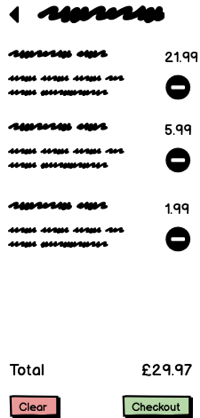
\includegraphics[width=0.45\columnwidth]{Figure1A.png}
	~~~
	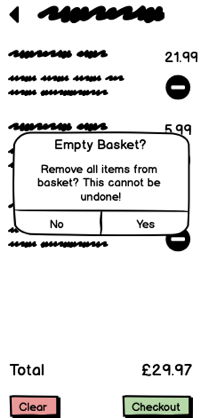
\includegraphics[width=0.45\columnwidth]{Figure1B.png}
	\caption{This is an example of a figure with a caption}
	\label{fig:example}
\end{figure}


\end{document}
